
\part{燃烧与燃烧室}

\begin{tcolorbox}
    针对常用的航空燃气涡轮发动机,请回答并分析以下问题:
    \begin{enumerate}
        \item 请以一款典型航空燃气涡轮发动机为例(可参考 CFM56,GE90,F119,M88
        ,EJ200, RB199, AL-31F 等),说明主燃烧室和加力燃烧室的燃烧组织技术,包括
        但不限于诸如扩压、火焰稳定、燃油喷射、流量分配、混合的设计方法与形式。
        \item 分析总结主燃烧室与加力燃烧室在设计中的异同;
        \item 总结近五十年来国际国内主燃烧室和加力燃烧室的出口温度水平与推力水平,
        并图示。
    \end{enumerate}
\end{tcolorbox}

\section{第一题}

本节以 CFM56 为例简单介绍燃烧室中的燃烧组织技术。
CFM56 是 CFM 国际公司设计的一款高涵道比涡轮风扇发动机,是世界上使用最广泛的涡扇发动机之一,安装于波音 737 及空中客车 A320 等客机上。

\begin{figure}[!ht]
    \centering
    \begin{subfigure}{0.5\linewidth}
        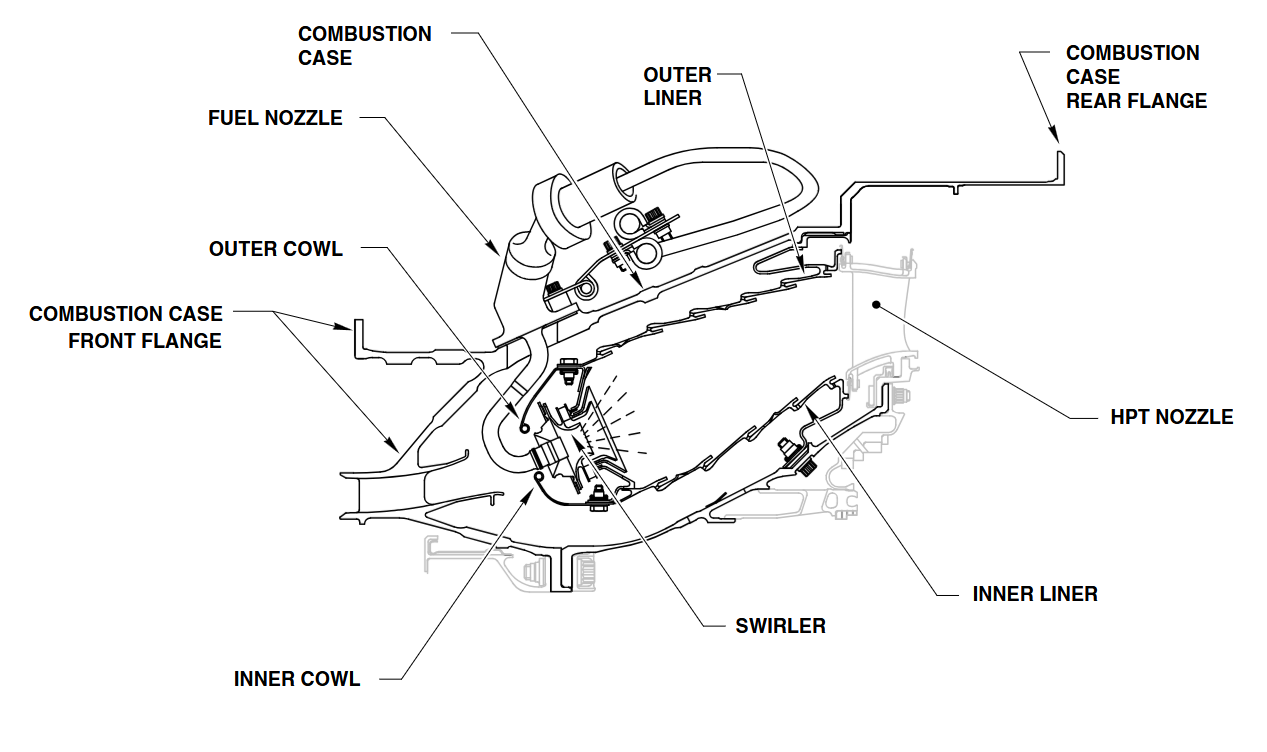
\includegraphics[width=\linewidth]{combustor-1.png}
        \caption{单环形燃烧室}
    \end{subfigure}
    \hfil
    \begin{subfigure}{0.45\linewidth}
        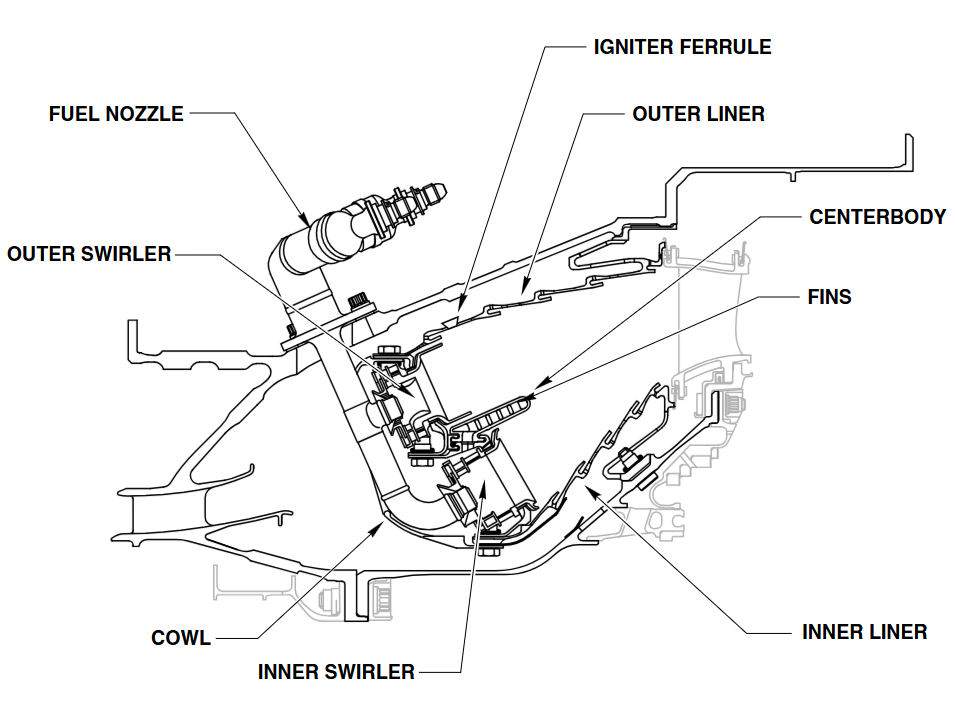
\includegraphics[width=\linewidth]{combustor-2.png}
        \caption{双环形燃烧室}
    \end{subfigure}
    \caption[CFM56 中使用的两种燃烧室截面图。]{CFM56 中使用的两种燃烧室截面图。}
    \label{fig:part-3-combustor}
    \textit{\small 来源:CFM56 维护训练手册}
\end{figure}

CFM56 上只安装了一个主燃烧室,其有多种设计方式,包括管形燃烧室或环管形燃烧室等,但是安装最广泛的版本使用的是环形燃烧室。
其上安装的环形燃烧室也分为单环形燃烧室和双环形燃烧室两种,主流的燃烧室设计是前者,而双环形燃烧室则可在高推力工况下使用双燃烧室,从而降低污染物的排放。

扩压器(Diffuser)是在燃烧室之前通过降低气体流速以提高压强的部件,在图~\ref{fig:part-3-combustor}中体现为入口后燃烧室腔的突然膨胀,这种扩压器称为突扩扩压器(Step diffuser)。
部分燃烧室的进气道会在气体流动方向上扩张,这种扩压器称为前置扩压器(Prediffuser)。
扩压可将压气机出口的气体中的动压恢复为静压,从而降低燃烧室的压力损失并缩小燃烧室的长度,提高燃烧效率。
另一方面,由于部分高速空气需从火焰筒上的孔中通过射流掺混,未经扩压的空气静压不足,会影响空气流量,从而影响燃烧。
针对扩压器的设计,一般要求其压力损失低、长度短、前置扩压器无分离、出口气流在周向和径向均匀、在所有工况下运行稳定且对压气机出口流场变化不敏感。

\begin{figure}[!ht]
    \centering
    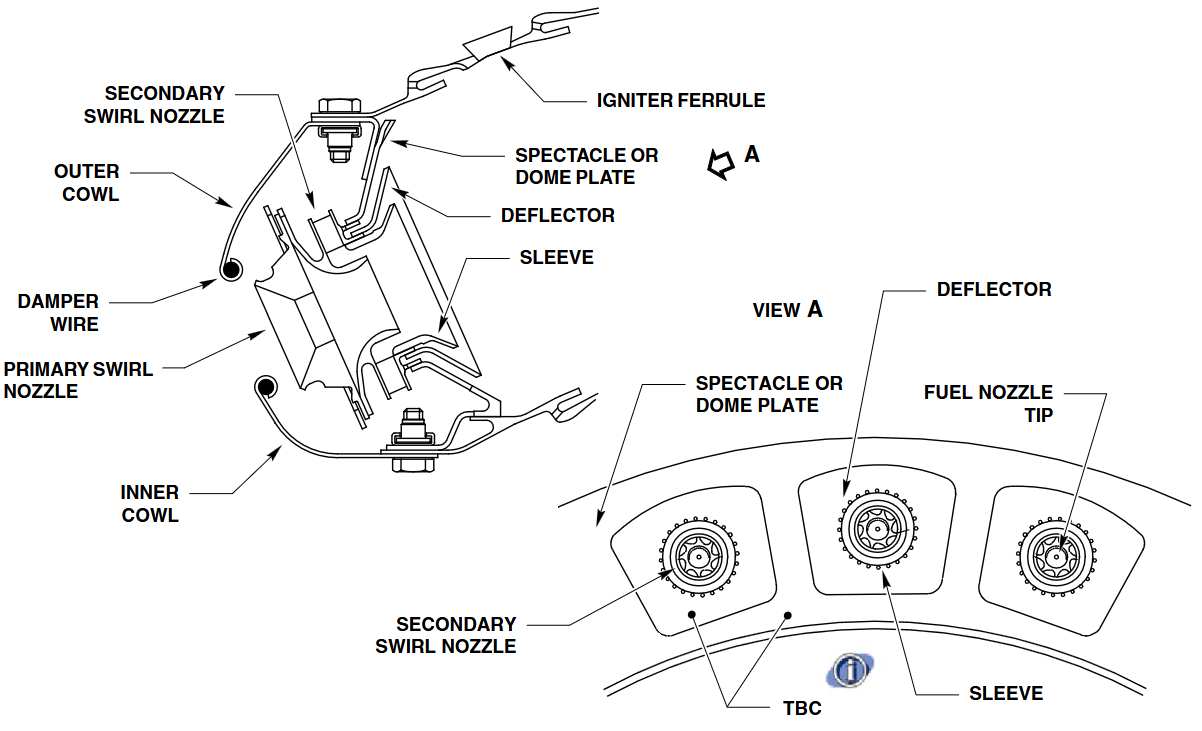
\includegraphics[width=0.8\linewidth]{combustor-nozzle.png}
    \caption{CFM56 单环形燃烧室喷嘴附近细节图。}
    \label{fig:part-3-combustor-nozzle}
    \textit{\small 来源:CFM56 维护训练手册}
\end{figure}

火焰稳定性是燃烧室设计的重要指标之一,而影响火焰稳定的重要参数是主燃区中,即紧邻燃料喷嘴的燃烧区域中,的空气流动。
通过操作空气流动以保证火焰稳定的主要方式是在喷嘴周围安装旋流器(Swirler,参见图~\ref{fig:part-3-combustor}),在主燃区形成回流区。
旋流器有径向和轴向两种设计方式,在此基础上还有多级的旋流器设计。
如图~\ref{fig:part-3-combustor-nozzle}所示,CFM56 燃烧室中的旋流器采用两级设计,主旋流器直接从轴向进气,而副旋流器则从侧向进气。
旋流器能够使气流高速旋转,产生强旋流流场,从而在旋流器出口附近形成一块空气反向流动的区域,称为回流区。
回流的气体中充满高温燃烧产物,因此可提供自动点火源,维持火焰稳定;此外,回流区中还具有流动速度较低的低速区。
因此,在回流区内进行的燃烧因此具有较好的火焰稳定性以及混合效果。
